\documentclass{article}
\usepackage{xeCJK}
\setCJKmainfont[BoldFont={WenQuanYi Zen Hei}, ItalicFont={WenQuanYi Zen Hei}]{WenQuanYi Zen Hei Mono}
\usepackage{geometry}
\usepackage{graphicx}
\usepackage{mathtools}
\usepackage[sc,osf,slantedGreek]{mathpazo}
\usepackage{color}
\usepackage{listings}
\lstdefinestyle{customc}{
  belowcaptionskip=1\baselineskip,
  breaklines=true,
  frame=L,
  xleftmargin=\parindent,
  language=C,
  showstringspaces=false,
  basicstyle=\footnotesize\ttfamily,
  keywordstyle=\bfseries\color{green},
  commentstyle=\itshape\color{purple!40!black},
  commentstyle=\color{red},
  identifierstyle=\color{blue},
  stringstyle=\color{orange},
}
\lstset{escapechar=@,style=customc}

%\usepackage[hidelinks,linkcolor=red]{hyperref}

\begin{document}
\title{Aho-Corasick Automaton Introduction}
\author{}
\maketitle

\section{Introduction}
The behaviour of the pattern matching machine is dictated by three functions: a goto function $g$, a failure function $f$, and an output function $output$

\begin{figure}[h]
  \centering
\caption{\textsc{Pattern matching machine}}
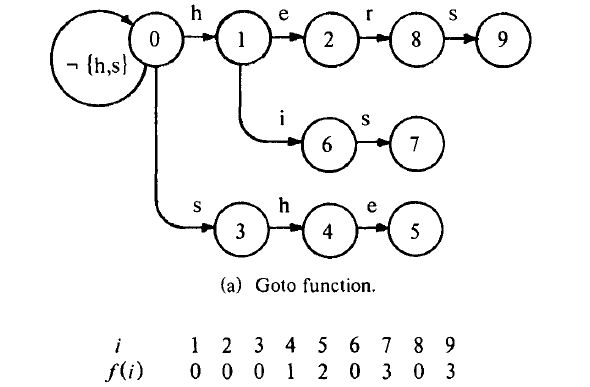
\includegraphics[scale=0.6]{res/ac.png}
\end{figure}

现在让我们来定义这三个函数,$goto$函数将一个状态和一个输入映射到另一个状态或\emph{fail},称之为状态跃迁(\textit{goto transition})。$failure$函数将一个状态映射到另一个状态,当$goto$函数返回\emph{fail}时调用(consulted)。$output$函数将一个状态关联到一个关键字集合或空。
\begin{align*}
goto    &:= (s,a) \mapsto
\begin{cases}
 s' \\
fail & \quad \text{ (the absense of an arrow)}
\end{cases}\\
f       &:= (s) \mapsto s'\\
output  &:= (s) \mapsto \{patterns\} \quad \text{ (associate a set of keywords or empty)}\\
\end{align*}

\section{Implementation}
\label{impl}
AC算法的实现有多种变体,基本在snort的源代码中都能找到,典型的实现包括$AC^{STD}$,也称作$AC_{v1}$定义于acsmx.c中。其他3种包括:$AC^{FULL}$, $AC^{Sparse}$, $AC^{Banded}$,也叫做$AC_{v2}$定义于acsmx2.c,即版本2。另外还有基于$AC^{FULL}$的变体$AC^{FULL\_Q}$,基于$AC^{Sparse}$和$AC^{Banded}$的变体$AC^{SPARSE\_BANDS}$。这里\texttt{Full, Sparse, Banded, SparseBanded}表示存储格式,以下为具体描述:
\begin{description}
\item[AC\_STD] \hfill \\
标准AC实现,即基于AC最初的论文\ref{1}实现的DFA,而实现的方法又决定着状态机的性能。我参考snort中acsmx.c(即AC实现第一版),通过以下结构存储AC状态机的状态跃迁表:
\begin{lstlisting}
typedef struct  {
    int      NextState[ ALPHABET_SIZE ];
    int      FailState;
    ACSM_PATTERN *MatchList;
}ACSM_STATETABLE;
\end{lstlisting}
\item[AC\_FULL] \hfill \\
$AC^{FULL}$属于$AC_{v2}$的一种,$AC_{v2}$对上述$AC^{STD}$的存储方案进行了优化,将上面的\lstinline|ACSM_STATETABLE|分解为每状态的状态跃迁表\lstinline|acsmTransTable|),每状态匹配表\lstinline|acsmMatchList|和用于NFA的每状态矢效指针\lstinline|acsmFailState|,见以下结构\lstinline|AC_STRUCT2|。\\为了方便描述,在之后的段落中我将忽略前缀\lstinline|acsm|,如\lstinline|TransTable|表示\lstinline|AC_STRUCT2|中的\lstinline|acsmTransTable|。
对于所有的$AC_{v2}$实现,都将先完成\lstinline|TransTable|的构建,即生成标准的DFA或NFA。然后,对于不同的存储格式,将\lstinline|TransTable|转化为\lstinline|NextState|。以下四种实现都是基于此实现,将\lstinline|TransTable|转化为Full, Sparse或Banded…
\begin{lstlisting}
typedef struct trans_node_s {
  acstate_t    key; // input symbol
  acstate_t    next_state;
  struct trans_node_s * next; /* next transition for this state */
} trans_node_t;

typedef struct {
    int acsmMaxStates; // 可能的最大状态
    int acsmNumStates; // 有效状态总数,active state
    ACSM_PATTERN2    * acsmPatterns;//关键字列表
//per-state failure state, used for build NFA
    acstate_t        * acsmFailState;

// 每个状态对应一个MatchList
    ACSM_PATTERN2   ** acsmMatchList;
// 基于链表的状态跃迁表,用于创建NFA和DFA,当构建完成,将其转化为full format matrix然后将内存释放
    trans_node_t ** acsmTransTable;
// 单独的状态跃迁表
    acstate_t ** acsmNextState;
...
} ACSM_STRUCT2;
\end{lstlisting}
\item[AC\_FULLQ] \hfill \\
  ditto, but matching states are queued
\item[AC\_SPARSE] \hfill \\
  Sparse matrix
\item[AC\_BANDED] \hfill \\
  Banded matrix
\item[AC\_SPARSEBANDS] \hfill \\
  Sparse-Banded matrix
\end{description}

\section{Principle}

\subsection{Construct goto}
为了理解Snort对标准实现的改进及改进所用的数据结构,我们以$AC^{FULL}$为例,构建goto function,下图描述了TransTable的变化。\\
仍然假设M表示模式匹配状态机,其中形如\texttt{'1: (I->6) -> (E->2)'}中的1表示M的当前状态为1,这行的意义是
\begin{align*}
g(1,a) =
\begin{cases}
6 & \quad \text{ if input symbol is i}\\
2 & \quad \text{ if input symbol is e}\\
\end{cases}
\end{align*}
 $g(1,a) $
从代码的角度解释:
其中1表示TransTable的index,\texttt{'1: (I->6) -> (E->2)'}表示\lstinline$TransTable[1]$对应链表(\lstinline$trans_node_t$),\texttt{'(I->6)'}表示链接的头节点\lstinline$node->key=i, node->next_state=6, node->next -> (E,2)$。注意:这里\underline{不区别大小写},下同

\begin{figure}[h]
  \centering
\caption{\textsc{goto corresponding to $AC_{v2}$}}
\begin{verbatim}
-- Add "he", TransTable(NumStates:2) --       -- Add "she", TransTable(NumStates:5) --
  0: (H->1)                                    0: (S->3) -> (H->1)
  1: (E->2)                                    1: (E->2)
                                               2:
                                               3: (H->4)
                                               4: (E->5)
-- Add "his", TransTable(NumStates:7) --      -- Add "hers", TransTable(NumStates:9) --
  0: (S->3) -> (H->1)                          0: (S->3) -> (H->1)
  1: (I->6) -> (E->2)                          1: (I->6) -> (E->2)
  2:                                           2: (R->8)
  3: (H->4)                                    3: (H->4)
  4: (E->5)                                    4: (E->5)
  5:                                           5:
  6: (S->7)                                    6: (S->7)
                                               7:
                                               8: (S->9)
\end{verbatim}
\end{figure}

\subsection{Build NFA}
\begin{enumerate}
  \item Make $f(s) = 0$ for all $s$ of depth 1
  \item 假设所有深度小于$d$的failure状态都已计算过了,则深度$d$的failure状态通过深度为$d-1$ goto的nonfail值确定。其中$d-1$的状态$r$,过程如下:
 \begin{enumerate}
    \item $g(r,a) == fail$ for all $a$, do nothing
    \item 否则当$g(r, a) = s$,$s$不为fail
      \begin{enumerate}
        \item state = f(r)
        \item while(g(state, a) != fail) state = f(state)
        \item set f(s) = g(state,a)
      \end{enumerate}
 \end{enumerate}
\end{enumerate}

\begin{lstlisting}
foreach(allsymbols as a)
  if ((s = goto(r,a)) != fail)
    state = f(r);
    while(goto(state,a) != fail)
      state = goto(state,a);
    f(s) = state;
\end{lstlisting}

\textbf{Examples}:
\begin{list}{}{}
  \item  f(1) = f(3) = 0
  \item  state 2: g(1,e) = 2(s); state=f(1)=0, while( (g(0,e) = 0) != fail) so f(s=2) = g(0,e) = 0
  \item  state 4: g(3,h) = 4(s); state=f(3)=0; while( (g(0,h) = 1) != fail) so f(s=4) = g(0,h) = 1
\end{list}
至此,我们生成了一个NFA,如下图所示:
\begin{figure}[h]
  \centering
  \caption{final fail function}
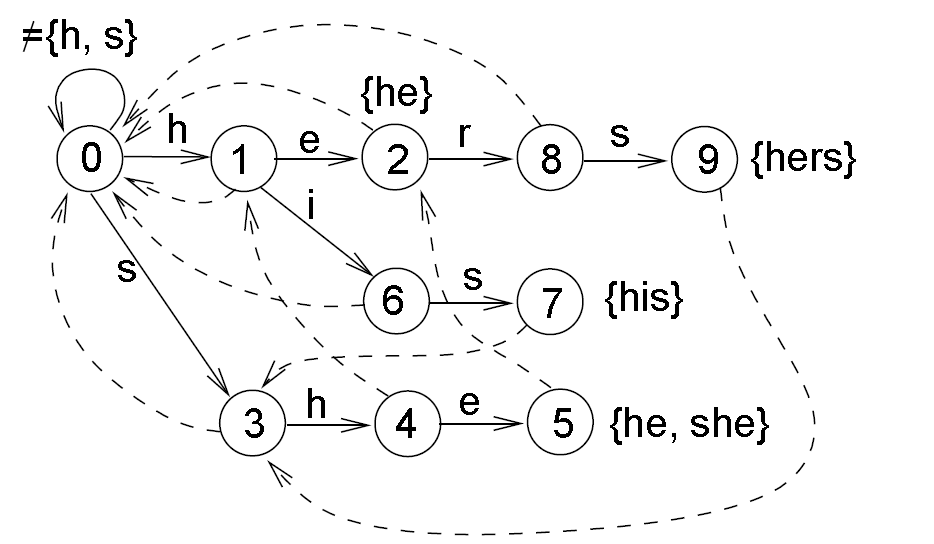
\includegraphics[scale=0.6]{res/failure.png}
\end{figure}
\subsection{Convert NFA to DFA}

通过以上算法生成的failure function在以下情况不是最优的:
设模式匹配状态机M,我们有$g(4,e) = 5$
如果M当前状态为4并且当前输入为$a_i$非$e$,则M将进入状态$f(4)=1$。因为M已经知道$a_i \ne e$,M无需考虑goto在状态为1输入为$e$时的值$g(1,e)$。事实上,如果关键字”his”不在,M可以直接的从状态4进入状态0,跳过多余的中间转移到状态1。\\
为了完全避免\textit{failure transitions},我们定义DFA版本的算法:
\textbf{DFA}(deterministic finite automaton)包含一个有限的状态集$S$和一个\textit{next move} function $\delta$ s.t. $\forall a, \delta(s,a) \in S$. 也就是说,DFA使每一输入精确的与一个状态对应。\\
我们可以通过以下算法将NFA中的goto和failure生成\textit{next move function} $\delta$:
\begin{lstlisting}
queue = empty
foreach(symbols as a)
  delta(0,a) = g(0,a)
  if g(0,a) != 0 then queue.push(g(0,a))

while !queue.empty()
  r = queue.front(); queue.pop();
  foreach(symbols as a)
    if(g(r,a) = s != fail
      queue.push(s)
      delta{r,a} = s
    else
      delta(r,a) = delta(f(r),a)
\end{lstlisting}

DFA和NFA最大的区别在于DFA能够\textbf{精确的}将每一个输入映射在有限集$S$中,NFA则需中间状态的过渡。

仍然以$AC^{FULL}$为例,通过以上算法得到的将NFA转化为DFA的结果如下,在M的任何一个状态下,每一个输入都有一个确定的next state,例如在M状态为3时我们有:
\begin{verbatim}
    input symbol     next state
    s                3
    h                4
    \neg{s,h}        0
\end{verbatim}
从NFA转化为DFA后的TransTable
\begin{verbatim}
  0: (S->3) -> (H->1)
  1: (S->3) -> (H->1) -> (I->6) -> (E->2)
  2: (S->3) -> (H->1) -> (R->8)
  3: (S->3) -> (H->4)
  4: (S->3) -> (I->6) -> (H->1) -> (E->5)
  5: (S->3) -> (R->8) -> (H->1)
  6: (H->1) -> (S->7)
  7: (S->3) -> (H->4)
  8: (H->1) -> (S->9)
  9: (S->3) -> (H->4)
\end{verbatim}


\section{Implementation Again}
前面一章讲到AC算法的全部原理,对于实现高效的$AC^{STD}$足矣,但是$AC^{STD}$会占用太多的内存,$AC_{v2}$主要的优化在于对存储结构的优化,其中不乏动用\textit{sparse matrix}和\textit{banded matrix},接下来我们首先来看看snort最简单的优化\textit{full matrix}版的AC实现$AC^{FULL}$。\\
前一章得到的DFA存储在\lstinline|TransTable|中,生成\textit{full matrix}的过程就是将转换为\lstinline|NextState|的过程,其实现通过\lstinline|Conv_List_To_Full|函数完成,其主要过程如下
\begin{lstlisting}
foreach(state as k)
    p = allocate(sizeofstate*(AlphabetSize+2), sizeofstate);
    trans_node_t *t = TransTable[k];
    p += 2;
    while (t != NULL)
      *((type_t *)p + t->key) = (type_t)t->next_state;
      t = t->next;
    p[0] = ACF_FULL;  // set format
    p[1] = 0;
    NextState[k] = p
\end{lstlisting}

最终生成的\textit{full matrix}如下所示:
\begin{figure}[h]
  \centering
\caption{\textsc{DFA in Full Matrix}}
\begin{verbatim}
Print DFA - 10 active states
   0: -> (I->1) -> (T->3)
   1: -> (F->2) -> (I->1) -> (J->6) -> (T->3)
   2: -> (I->1) -> (S->8) -> (T->3) HE
   3: -> (I->4) -> (T->3)
   4: -> (F->5) -> (I->1) -> (J->6) -> (T->3)
   5: -> (I->1) -> (S->8) -> (T->3) HE SHE
   6: -> (I->1) -> (T->7)
   7: -> (I->4) -> (T->3) HIS
   8: -> (I->1) -> (T->9)
   9: -> (I->4) -> (T->3) HERS
\end{verbatim}
\end{figure}


\begin{thebibliography}{99}
\bibitem[1]{1} Efficient String matching: An Aid to Bibliographic Search
\bibitem[2]{2} Optimizing Pattern Matching for Intrusion Detection
\end{thebibliography}
\end{document}

%%% Local Variables:
%%% mode: latex
%%% TeX-master: t
%%% End:
